% TG-LiteNet -- CSD361 final report (IEEE conference format, <= 8 pages).
% Build:   python scripts/make_report_assets.py   (fills report/generated/ from results/)   then   pdflatex main; bibtex-free (thebibliography inline).
% Set \drafttrue -> \draftfalse before submitting: it hides every red TODO marker.
\documentclass[conference]{IEEEtran}
\IEEEoverridecommandlockouts
\setlength{\textfloatsep}{8pt plus 2pt minus 2pt}\setlength{\floatsep}{8pt plus 2pt minus 2pt}\setlength{\intextsep}{8pt plus 2pt minus 2pt}
\usepackage{cite}
\usepackage{amsmath,amssymb,amsfonts}
\usepackage{algorithmic}
\usepackage{algorithm}
\usepackage{graphicx}
\usepackage{textcomp}
\usepackage{xcolor}
\usepackage{booktabs}
\usepackage{multirow}
\usepackage{adjustbox}
\usepackage{url}
\usepackage{tikz}
\usetikzlibrary{arrows.meta,positioning,shapes.geometric,fit,backgrounds}
\def\BibTeX{{\rm B\kern-.05em{\sc i\kern-.025em b}\kern-.08em T\kern-.1667em\lower.7ex\hbox{E}\kern-.125em X}}

% ---------------------------------------------------------------- draft helpers
\newif\ifdraft \draftfalse
\newcommand{\todo}[1]{\ifdraft{\color{red}[TODO: #1]}\fi}
\newcommand{\safefig}[2]{% width, file (no extension)
  \IfFileExists{figures/#2.pdf}{\includegraphics[width=#1]{figures/#2.pdf}}{%
  \IfFileExists{figures/#2.png}{\includegraphics[width=#1]{figures/#2.png}}{%
  \fbox{\parbox{#1}{\centering\footnotesize\color{red}[figure \detokenize{#2} missing -- run scripts/make\_report\_assets.py]}}}}\par}
% auto-generated by scripts/make_report_assets.py - do not edit
\newcommand{\srcDiceA}{0.830}
\newcommand{\unDiceA}{0.762}
\newcommand{\unClA}{0.835}
\newcommand{\unBettiA}{75.0}
\newcommand{\gapDiceA}{0.068}
\newcommand{\srcDiceD}{0.822}
\newcommand{\unDiceD}{0.757}
\newcommand{\unClD}{0.832}
\newcommand{\unBettiD}{44.7}
\newcommand{\gapDiceD}{0.065}
\newcommand{\srcDiceE}{0.822}
\newcommand{\unDiceE}{0.756}
\newcommand{\unClE}{0.833}
\newcommand{\unBettiE}{42.7}
\newcommand{\gapDiceE}{0.066}
\newcommand{\paramsA}{31.04}
\newcommand{\gflopsA}{384.7}
\newcommand{\cpumsA}{2915}
\newcommand{\paramsE}{0.21}
\newcommand{\gflopsE}{5.5}
\newcommand{\cpumsE}{429}
\newcommand{\paramRatio}{147}
\newcommand{\flopRatio}{70}
\newcommand{\hwGPU}{Tesla T4}
\newcommand{\hwCPU}{x86\_64}
\newcommand{\hwTorch}{2.11.0+cu128}
\newcommand{\nSeeds}{5}
            % \srcDiceA, \unDiceE, \paramsE, ... (XX until results exist)
\IfFileExists{generated/numbers.tex}{}{\typeout{numbers.tex missing}}

\DeclareMathOperator*{\argmin}{arg\,min}
\newcommand{\cl}{\mathrm{clDice}}

\renewcommand{\IEEEkeywordsname}{Keywords}
\begin{document}

\title{TG-LiteNet: A Topology-Preserving, Domain-Generalizable and Lightweight Framework for Retinal Vessel Segmentation in Resource-Constrained Screening Settings\\
\large CSD361 -- Introduction to Machine Learning, Final Project Report}

\author{\IEEEauthorblockN{Abhiraj Agarwal}
\IEEEauthorblockA{Roll No.\ 2510110002}
\and
\IEEEauthorblockN{Shashwat Rajan}
\IEEEauthorblockA{Roll No.\ 2510111019}
\and
\IEEEauthorblockN{Tanish Shitanshu}
\IEEEauthorblockA{Roll No.\ 2510110008}
\\
\IEEEauthorblockA{Department of Computer Science and Engineering, Shiv Nadar Institution of Eminence, Delhi NCR, India}}

\maketitle

% =============================================================================== ABSTRACT
\begin{abstract}
Retinal vessel segmentation underpins screening for diabetic retinopathy, glaucoma and hypertensive retinopathy, but a model deployed in a rural screening camp must (i) keep thin vessels \emph{connected}, (ii) work on cameras it was never trained on, and (iii) run on modest hardware. Published work usually optimises at most two of these three properties and rarely reports them together under one protocol. We study the three-way trade-off with \emph{TG-LiteNet}, a compact depthwise-separable encoder--decoder trained on a single source dataset (DRIVE) with a soft-clDice topology loss, an auxiliary skeleton head, lightweight style-and-structure augmentation with a consistency loss, and Monte-Carlo-dropout uncertainty. A staged ablation (U-Net $\rightarrow$ +topology $\rightarrow$ +DG $\rightarrow$ +compact backbone $\rightarrow$ +uncertainty) with \nSeeds\ seeds per stage, a full $2{\times}2{\times}2$ factorial design and capacity/loss-variant sweeps are evaluated on three held-out target datasets (STARE, CHASE\_DB1, HRF) using Dice, clDice, Betti-number error, the source-to-target gap, parameters, FLOPs, latency and uncertainty--error correlation. TG-LiteNet has \paramsE\,M parameters and \gflopsE\,GFLOPs (U-Net: \paramsA\,M, \gflopsA\,GFLOPs; a factor of \paramRatio\ in parameters and \flopRatio\ in FLOPs) and reaches an unseen-domain Dice of \unDiceE\ and clDice of \unClE, versus \unDiceA\ and \unClA\ for the U-Net baseline. Topology supervision more than halves the unseen Betti-0 error of the U-Net (\unBettiA\ to 30.2) at a cost of about 0.01 Dice, DG augmentation recovers about 0.01 unseen Dice, and the compact backbone stays within 0.005 Dice of the U-Net (a small but consistent loss) and gives back about half of the topology gain (Betti-0 error \unBettiE). MC-dropout uncertainty ranks pixel errors moderately ($\rho_{px}\approx0.31$--$0.34$), but image-level rejection is not reliably better than random. All numbers are produced by the released code; no target-domain image or label is used for training, tuning or model selection.
\end{abstract}

\begin{IEEEkeywords}
retinal vessel segmentation, topology-preserving loss, domain generalization, lightweight networks, uncertainty estimation, DRIVE
\end{IEEEkeywords}

% =============================================================================== I. INTRODUCTION
\section{Introduction}
Segmenting the retinal vascular tree from fundus photographs supports the measurement of vessel calibre, tortuosity and branching used in screening for diabetic retinopathy, glaucoma and hypertensive retinopathy~\cite{liu2025review}. Since U-Net~\cite{ronneberger2015} such networks are trained and tested on small public datasets, typically DRIVE~\cite{staal2004}, STARE~\cite{hoover2000}, CHASE\_DB1~\cite{fraz2012} and HRF~\cite{budai2013}. Overlap scores hide topological errors: a single severed centreline barely changes Dice but changes the connectivity that downstream biomarkers rely on~\cite{shit2021,shi2024,kirchhoff2024}.

\textbf{Motivation.} A model that is useful in a low-resource screening programme must satisfy three constraints \emph{simultaneously}: it must preserve vessel \emph{topology}; it must tolerate camera and population \emph{shift}, ideally without target labels, because performance falls when a model meets a new database~\cite{galdran2022,fadugba2024}; and it must be small and fast enough for \emph{edge} hardware~\cite{sobhan2026}, as in screening camps with limited compute and connectivity. Recent papers each address part of this, so our contribution is not a simple ``combination of the three''.

\textbf{Problem statement.} Let $f_\theta$ be trained on a labelled source domain $\mathcal S$ (DRIVE) and evaluated, with no access to target images or labels, on unseen domains $\mathcal T=\{\text{STARE, CHASE\_DB1, HRF}\}$. For a metric $m$ the \emph{target gap} is $\Delta_m(\mathcal T)=m(\mathcal S)-m(\mathcal T)$. The goal is to keep $\Delta_m$ small for both overlap and topology metrics under a compact parameter and latency budget, and to flag unreliable predictions with an uncertainty estimate.

\textbf{Objectives.} (O1) Build a reproducible \emph{source-only} pipeline for topology-aware vessel segmentation; (O2) quantify what each component (topology loss, DG augmentation, compact backbone, uncertainty) contributes to accuracy, topology, cross-domain gap and cost in one controlled ablation; (O3) test whether MC-dropout uncertainty can triage unreliable predictions, especially on unseen domains.

\textbf{Approach and contributions.} We propose \emph{TG-LiteNet}, a depthwise-separable encoder--decoder with a mask head and an auxiliary skeleton head. Our contributions are: (1) a staged ablation and a full $2{\times}2{\times}2$ factorial study (backbone $\times$ topology loss $\times$ DG augmentation) measured with repeated seeds and confidence intervals; (2) a unified evaluation that reports Dice/IoU, clDice, Betti-0/1 error, the source-to-target gap, total parameters, FLOPs, CPU/GPU latency and uncertainty quality \emph{together}; (3) an uncertainty-based triage analysis at pixel and image level, separately for the source and each unseen domain; and (4) open code that regenerates every number in this paper. We do not claim a new loss or a new architecture family, and we make no state-of-the-art claim.

% =============================================================================== II. RELATED WORK
\section{Related Work}
\textbf{Base paper: clDice.} Shit et al.~\cite{shit2021} compare the skeleton of a prediction with the ground-truth mask (topology precision) and the skeleton of the ground truth with the predicted mask (topology sensitivity); their harmonic mean is clDice. They prove that maximising clDice preserves topology up to homotopy equivalence for binary tubular structures and give a differentiable \emph{soft-clDice} based on iterated soft morphological opening. On five datasets, including DRIVE, clDice-trained networks reduce Betti errors at a small training-time overhead. cbDice~\cite{shi2024} observes that clDice favours large vessels (``diameter imbalance'') and adds radius and boundary information; Skeleton Recall Loss~\cite{kirchhoff2024} computes the skeleton once, offline, with cheap CPU operations; earlier work used persistent homology~\cite{hu2019}. None of these is evaluated for source-only robustness under dataset shift.

\textbf{Domain generalisation and adaptation.} ``Cross-dataset'' covers four protocols: source-only transfer, multi-source DG, test-time adaptation (TTA) and fine-tuning with target labels. DGSSA~\cite{liu2026dgssa} synthesises vessel trees by space colonisation and adds style augmentation (multi-source); WaveRNet~\cite{wang2026wavernet} separates illumination-robust low frequencies with a SAM backbone; Hu et al.~\cite{hu2024hessian} and GraphSeg~\cite{liu2025graphseg} use a Hessian vector field and a deformable graph prior. A benchmark~\cite{fadugba2024} finds that, with enough training data, a plain U-Net generalises well.

\textbf{Lightweight networks.} Galdran et al.~\cite{galdran2022} show that U-Nets with $\sim$34K and W-Nets with $\sim$68K parameters are competitive; DSAE-Net~\cite{zeng2025} (78K parameters, skeleton-distance loss) and LightVesselNet~\cite{sobhan2026} (75K parameters) report cross-dataset Dice but no connectivity metrics or uncertainty; a reverse-attention U-Net~\cite{hernandez2025} targets embedded use.

\textbf{Topology under shift; uncertainty.} TFFM~\cite{ahmed2026} (source-only transfer), TopoTTA~\cite{zhou2025}, TopoLoRA-SAM~\cite{khazem2026} and TAPDecoderFT~\cite{huang2026} report clDice/Betti after zero-shot, test-time or fine-tuned transfer, but with large or unspecified models and no latency. Topology-aware uncertainty~\cite{gupta2023} scores whole structures; MC dropout~\cite{gal2016} is a cheap pixel-level alternative whose quality degrades under dataset shift~\cite{ovadia2019}.

\textbf{Research gap.} Table~\ref{tab:gap} summarises what the closest works report. Among the works we reviewed, none evaluates a compact \emph{source-only} model for topology, total deployment cost and uncertainty quality in one controlled protocol with repeated runs. This project fills exactly that gap, as a trade-off \emph{study} rather than a new method.

\begin{table}[t]
\centering
\caption{Evidence reported by the closest reviewed works (\checkmark: reported, $\sim$: partial/indirect, --: not reported). Protocol: SO = source-only, MS = multi-source DG, TTA, FT = fine-tuning on labelled target data.}
\label{tab:gap}
\footnotesize
\setlength{\tabcolsep}{3pt}
\begin{adjustbox}{max width=\columnwidth}\begin{tabular}{l c c c c c}
\toprule
Work & Protocol & Topo.\ loss & Topo.\ metrics & Total cost & Uncert. \\
\midrule
clDice / SRL~\cite{shit2021,kirchhoff2024} & none & \checkmark & \checkmark & $\sim$ & -- \\
DGSSA, WaveRNet~\cite{liu2026dgssa,wang2026wavernet} & MS & -- & -- & -- & -- \\
Minimal., DSAE, LightVessel~\cite{galdran2022,zeng2025,sobhan2026} & train 1, test many & $\sim$ & -- & \checkmark & -- \\
TFFM~\cite{ahmed2026} & SO & \checkmark & \checkmark & -- & -- \\
TopoTTA~\cite{zhou2025} & TTA & $\sim$ & \checkmark & n/v & -- \\
TopoLoRA-SAM, TAPDecoderFT~\cite{khazem2026,huang2026} & FT & \checkmark & \checkmark & $\sim$ & -- \\
Topology-aware unc.~\cite{gupta2023} & -- & -- & $\sim$ & n/v & \checkmark \\
\midrule
\textbf{TG-LiteNet (this work)} & SO & \checkmark & \checkmark & \checkmark & \checkmark \\
\bottomrule
\end{tabular}\end{adjustbox}
\end{table}

% =============================================================================== III. PROBLEM FORMULATION
\section{Problem Formulation and Research Questions}
Given a fundus image $I$ with field-of-view (FOV) mask $F$, predict a binary vessel mask $M\in\{0,1\}^{H\times W}$. Models are trained on DRIVE only; STARE, CHASE\_DB1 and HRF are never used for training, tuning or model selection. We ask:
\begin{itemize}
\item \textbf{RQ1 (topology).} Does topology supervision (soft-clDice + skeleton head) improve clDice and Betti error relative to Dice+BCE without an unacceptable loss of overlap?
\item \textbf{RQ2 (generalisation).} Does lightweight style-plus-structure augmentation with a consistency loss reduce $\Delta_m$ from DRIVE to the unseen targets?
\item \textbf{RQ3 (trade-off).} What accuracy and topology cost does a $\le$2M-parameter budget incur relative to the savings in parameters, FLOPs and latency?
\item \textbf{RQ4 (uncertainty).} Does MC-dropout uncertainty rank high-error cases and support selective rejection, more so on unseen domains than on the source domain?
\end{itemize}

% =============================================================================== IV. METHOD
\section{Proposed Methodology}
\subsection{Overview}
Fig.~\ref{fig:pipeline} shows the pipeline. A fundus image is rescaled so that its FOV has a fixed width, reduced to the CLAHE-enhanced, standardised green channel, and passed through an encoder--decoder with a mask head (and, during training only, a skeleton head). The loss combines region, pixel, topology and consistency terms. At test time, $T$ stochastic forward passes give a mean probability map and a variance map used as uncertainty.

\begin{figure}[t]
\centering
\resizebox{\columnwidth}{!}{%
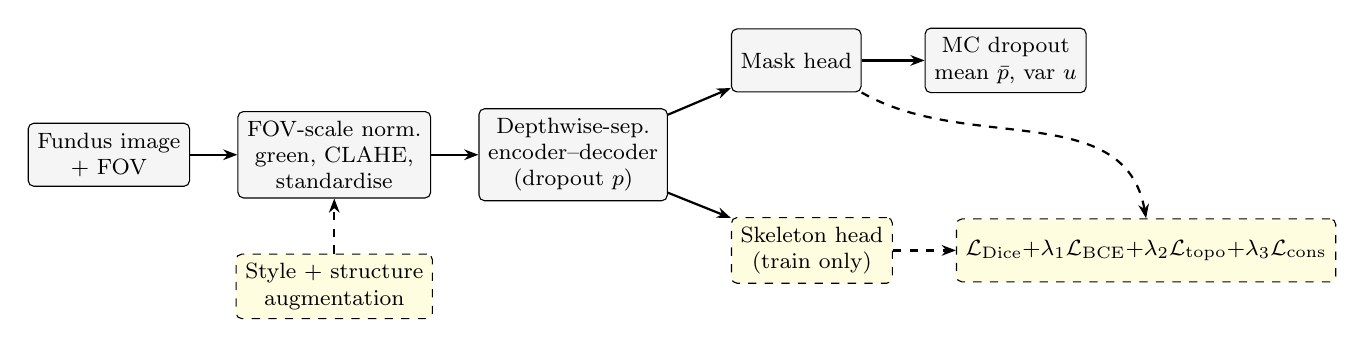
\begin{tikzpicture}[font=\footnotesize, node distance=5mm and 6mm,
  box/.style={draw, rounded corners=2pt, minimum height=8mm, align=center, fill=gray!8},
  tr/.style={draw, dashed, rounded corners=2pt, minimum height=8mm, align=center, fill=yellow!12},
  arr/.style={-{Stealth[length=1.8mm]}, thick}]
  \node[box] (img) {Fundus image\\+ FOV};
  \node[box, right=of img] (pre) {FOV-scale norm.\\green, CLAHE,\\standardise};
  \node[box, right=of pre] (net) {Depthwise-sep.\\encoder--decoder\\(dropout $p$)};
  \node[box, above right=2mm and 8mm of net] (mask) {Mask head};
  \node[tr, below right=2mm and 8mm of net] (skel) {Skeleton head\\(train only)};
  \node[box, right=8mm of mask] (mc) {MC dropout\\mean $\bar p$, var $u$};
  \node[tr, below=7mm of pre] (dg) {Style + structure\\augmentation};
  \node[tr, right=8mm of skel] (loss) {$\mathcal L_{\mathrm{Dice}}{+}\lambda_1\mathcal L_{\mathrm{BCE}}{+}\lambda_2\mathcal L_{\mathrm{topo}}{+}\lambda_3\mathcal L_{\mathrm{cons}}$};
  \draw[arr] (img) -- (pre); \draw[arr] (pre) -- (net);
  \draw[arr] (net) -- (mask); \draw[arr] (net) -- (skel);
  \draw[arr] (mask) -- (mc);
  \draw[arr, dashed] (dg) -- (pre);
  \draw[arr, dashed] (skel) -- (loss);
  \draw[arr, dashed] (mask.south east) to[out=-30,in=100] (loss.north);
\end{tikzpicture}}
\caption{TG-LiteNet pipeline. Dashed/yellow elements are used only during training; one fixed model is evaluated on every target.}
\label{fig:pipeline}
\end{figure}

\subsection{Preprocessing and scale normalisation}
Cameras differ strongly in resolution (HRF images are $\sim$6$\times$ wider than DRIVE's), so the pixel width of vessels, to which a convolutional model is very sensitive, changes with the dataset. Every image is rescaled so that its FOV is $W_F{=}527$\,px wide (DRIVE's median), which uses neither labels nor any statistic of the target \emph{dataset}. We then take the green channel (best vessel contrast), replace the outside of the FOV by the FOV mean, apply CLAHE~\cite{zuiderveld1994} with a fixed tile size in pixels, standardise inside the FOV, and set the outside to zero. The same deterministic function is used in training and testing.

\subsection{Architectures}
\textbf{Baseline U-Net}~\cite{ronneberger2015}: four 2$\times$2 max-pool stages, double 3$\times$3 conv+BN+ReLU blocks, transposed-convolution up-sampling, base width 64 ($\approx$\paramsA\,M parameters).

\textbf{TG-LiteNet backbone.} Every 3$\times$3 convolution is replaced by a depthwise 3$\times$3 followed by a pointwise 1$\times$1 convolution (BN, ReLU6), as in MobileNets~\cite{howard2017}. A block has two such layers and a 1$\times$1 residual shortcut. Encoder widths are $(w,2w,4w,8w,8w)$ with $w{=}16$; the decoder uses bilinear up-sampling, skip concatenation and one separable block per level. A $1{\times}1$ mask head outputs vessel logits; an auxiliary $1{\times}1$ skeleton head (training only, no inference cost) predicts the 1-px-dilated skeleton of the label. Spatial dropout ($p{=}0.1$) after the bottleneck and each decoder block is used only in stage E. The width $w$ is the single capacity knob; Section~\ref{sec:ablation} sweeps it.

\subsection{Objective}
For a prediction $P=\sigma(z)\in[0,1]^{H\times W}$, label $G$ and FOV $F$, the total loss is
\begin{equation}
\mathcal L=\mathcal L_{\mathrm{Dice}}+\lambda_1\mathcal L_{\mathrm{BCE}}+\lambda_2\mathcal L_{\mathrm{topo}}+\lambda_3\mathcal L_{\mathrm{cons}},
\label{eq:loss}
\end{equation}
with all terms computed inside $F$. $\mathcal L_{\mathrm{Dice}}$ and $\mathcal L_{\mathrm{BCE}}$ are the usual soft-Dice and binary cross-entropy.

\emph{Topology term.} With $S(\cdot)$ the (soft) morphological skeleton, topology precision and sensitivity are
$T_{\mathrm{prec}}=\frac{\sum S(P)\odot G}{\sum S(P)}$, $T_{\mathrm{sens}}=\frac{\sum S(G)\odot P}{\sum S(G)}$, and
\begin{equation}
\mathcal L_{\mathrm{clDice}}=1-\frac{2\,T_{\mathrm{prec}}T_{\mathrm{sens}}}{T_{\mathrm{prec}}+T_{\mathrm{sens}}}.
\end{equation}
$S(P)$ is the differentiable skeleton obtained by iterating soft erosion/opening (10 iterations, enough for vessels up to 10\,px radius at our scale); $S(G)$ is the exact skeleton of the (augmented) label, computed in the data loader. The skeleton head adds $\mathcal L_{\mathrm{skel}}=\mathrm{Dice}+\mathrm{BCE}$ against the dilated skeleton, so $\mathcal L_{\mathrm{topo}}=\mathcal L_{\mathrm{clDice}}+\gamma\mathcal L_{\mathrm{skel}}$. As supplementary variants we implemented the binary Skeleton Recall loss~\cite{kirchhoff2024}, $\mathcal L_{\mathrm{SR}}=1-\sum P\odot\mathcal T(S(G))/\sum\mathcal T(S(G))$ with $\mathcal T$ a 3$\times$3 dilation, and their sum. We also re-implemented the radius- and boundary-aware cbDice~\cite{shi2024} (the cl-MIN-Dice variant) from its equations: with $D$ the distance-to-boundary maps and $r$ the skeleton radii, $T_{\mathrm{prec}}=\sum_{S_P}\tfrac{D_L}{r_P}\big/\big(|S_P\setminus S_L|+\sum_{S_P\cap S_L}\tfrac{r_L}{r_P}\big)$ and symmetrically $T_{\mathrm{sens}}$, combined as in Eq.~(2). It coincides with clDice for aligned centrelines but gives only partial credit to a predicted centreline that is displaced inside the vessel, and is meant to be paired with Dice. The label's skeleton and distance map are exact; for the prediction we use the soft skeleton and a differentiable soft-erosion distance map (so it may differ numerically from the authors' code). cbDice is evaluated as a metric for every model and tested as a loss variant (Sec.~\ref{sec:ablation}).

\emph{Consistency term (DG).} For each patch we build a perturbed view $\tilde x$ (below) that is pixel-aligned with the clean view $x$:
$\mathcal L_{\mathrm{cons}}=\frac{1}{|F|}\sum_F\big(\sigma(f(\tilde x))-\mathrm{sg}[\sigma(f(x))]\big)^2$, where $\mathrm{sg}$ stops gradients. Both views are also supervised.

\subsection{Domain-generalisation augmentation}
All stages use the same standard geometric augmentation (random crop at a FOV pixel, flips, free rotation, isotropic scaling in $[0.8,1.25]$). Stage C onwards additionally applies, \emph{only at training time}: \textbf{style} --- random gain/gamma/contrast/brightness, smooth multiplicative illumination field, Gaussian blur, noise and JPEG compression of the green channel before CLAHE; and \textbf{structure} --- an elastic deformation applied identically to both views and the label, and local intensity dropout (soft ellipses with attenuated contrast, view 2 only). Because CLAHE and standardisation follow the colour/gamma/contrast jitter, those three perturbations are largely neutralised by design (the same pipeline runs at test time); the effective style perturbations are the illumination field, blur, noise and JPEG. A DG stage processes two views per patch (clean and perturbed), i.e.\ twice the forward passes of stages A/B for the same number of iterations and patches; the elastic warp is capped so that it never folds (positive Jacobian). This is deliberately much simpler than synthesising vessel trees~\cite{liu2026dgssa}.

\subsection{Uncertainty and triage}
With dropout kept active (BatchNorm in evaluation mode), $T$ passes give $p_t=\sigma(f_t(x))$, the mean $\bar p=\frac1T\sum_t p_t$ and the variance $u=\frac1T\sum_t p_t^2-\bar p^2$~\cite{gal2016}. We compare $u$ with the predictive entropy $H(\bar p)$, which is also available for deterministic models. For triage, an image is scored by its mean $u$ inside $F$; the images (or pixels) with the largest score are rejected first.

\begin{algorithm}[t]
\caption{Training one TG-LiteNet configuration (one seed)}
\label{alg:train}
\footnotesize
\begin{algorithmic}[1]
\STATE Pre-compute standardised green+CLAHE inputs of the 16 training images (DRIVE, scale-normalised)
\FOR{iteration $=1,\dots,N$}
  \STATE sample $B$ patches: random affine crop of $x$, label $G$, FOV $F$, exact skeleton $S(G)$
  \IF{DG enabled}\STATE $\tilde x\leftarrow$ style($x$) with the same crop/elastic warp; local intensity dropout\ENDIF
  \STATE forward ($x$ [and $\tilde x$]) $\rightarrow$ mask logits [and skeleton logits]
  \STATE $\mathcal L\leftarrow$ Eq.~\eqref{eq:loss} (terms enabled by the stage)
  \STATE AdamW step (cosine schedule, gradient clipping)
  \IF{iteration $\bmod$ $v=0$}\STATE evaluate Dice on the 4 DRIVE \emph{validation} images; keep the best checkpoint\ENDIF
\ENDFOR
\STATE \textbf{test:} evaluate the checkpoint on DRIVE-test, STARE, CHASE\_DB1, HRF (fixed threshold 0.5)
\end{algorithmic}
\end{algorithm}

% =============================================================================== V. EXPERIMENTAL SETUP
\section{Experimental Setup}\label{sec:setup}
\subsection{Datasets, preprocessing and exploratory analysis}
Table~\ref{tab:data} lists the datasets. DRIVE provides 20 training and 20 test images; we split the training images once (seed 2026) into 16 for training and 4 for validation (model selection and, if used, hyper-parameter selection), and use the 20 test images as the in-domain test set. STARE (20), CHASE\_DB1 (28) and HRF (45) are used only for testing. Ground truth is the first human observer. HRF and (when available) official DRIVE masks provide the FOV; for DRIVE (mirror), STARE and CHASE\_DB1 the FOV is estimated by thresholding, keeping the largest component and eroding it by 1\% (checked visually, Fig.~\ref{fig:data}). The vessel fraction is 9--13\% in every dataset, i.e.\ about 1:8 class imbalance; there are no missing values or categorical attributes in this task. The exploratory statistics of Table~\ref{tab:data} quantify the domain shift: the mean green-channel intensity ranges from $\approx$60 (CHASE\_DB1, HRF) to $\approx$110 (STARE), and while the vessel calibre after FOV normalisation is $\approx$3.5\,px for DRIVE, STARE and CHASE\_DB1, it is only $\approx$1.4\,px for HRF: HRF's reference annotations are thin relative to its field of view, so HRF measures an annotation-style shift in addition to the camera shift (we did not run a no-rescale evaluation; see Sec.~\ref{sec:limits}). DRIVE and CHASE\_DB1 were obtained from public mirrors (see \texttt{README.md}), STARE and HRF from the official sites; sources and checksums are recorded in \texttt{data/MANIFEST.json}.

\begin{table}[t]
\centering
\caption{Datasets (all statistics measured on the files used in our experiments). FOV = field-of-view width, used to normalise the scale of every image; calibre = mean vessel width (2$\times$ distance transform on the label skeleton) at native resolution and after normalisation to a 527\,px FOV; G = green-channel mean$\pm$std inside the FOV (0--255). Source = train (16) / validation (4) / test (20 official test images); targets are test-only.}
\label{tab:data}
\small
\begin{adjustbox}{max width=\columnwidth}\begin{tabular}{l r c r r c c l}
\toprule
Dataset & \# & Size (px) & Vessel \% & FOV (px) & Calibre (px) & G & Role \\
\midrule
DRIVE~\cite{staal2004} & 40 & 565$\times$584 & 12.9 & 527 & 3.5$\to$3.5 & 97$\pm$17 & source \\
STARE~\cite{hoover2000} & 20 & 700$\times$605 & 10.5 & 638 & 4.3$\to$3.5 & 109$\pm$24 & target \\
CHASE\_DB1~\cite{fraz2012} & 28 & 999$\times$960 & 10.3 & 899 & 6.1$\to$3.6 & 62$\pm$26 & target \\
HRF~\cite{budai2013} & 45 & 3504$\times$2336 & 9.1 & 3262 & 8.8$\to$1.4 & 60$\pm$17 & target \\
\bottomrule
\end{tabular}\end{adjustbox}
\end{table}

\begin{figure}[t]
\centering
\safefig{\columnwidth}{data_overview}
\caption{Exploratory view of the datasets: vessel labels (green) and FOV outlines (red). Camera, colour balance, field of view and resolution differ markedly between datasets, which is the domain shift studied here.}
\label{fig:data}
\end{figure}

\subsection{Implementation and procedure}
Everything is implemented in Python with PyTorch~\cite{paszke2019} (\hwTorch), OpenCV, scikit-image~\cite{vanderwalt2014} (Zhang--Suen thinning~\cite{zhang1984} for skeletons, connected components, Euler number) and scikit-learn. Training and efficiency measurements ran on free Kaggle notebooks with a \hwGPU\ GPU and a 4-thread \hwCPU\ CPU. All stages share the optimiser, schedule and data pipeline (Table~\ref{tab:hparams}); stages differ only in the switches of Table~\ref{tab:stages}. We train each stage A--E with \nSeeds\ seeds and each additional configuration (factorial cells, loss variants, widths) with 2 seeds, and report mean$\pm$std; differences between configurations are given with 95\% Welch intervals (computed on per-seed unseen averages; all intervals are in \texttt{results/tables/stage\_deltas.csv} and \texttt{factorial\_deltas.csv}).

\begin{table}[t]
\centering
\caption{Training configuration shared by all stages (generated from \texttt{configs/base.yaml}).}
\label{tab:hparams}
\small
\begin{adjustbox}{max width=\columnwidth}\begin{tabular}{ll}
\toprule
Item & Value \\
\midrule
Optimiser & AdamW, lr $0.001$, wd $0.0001$ \\
Schedule & 200 warm-up it., cosine to $1\%$ \\
Iterations / batch / patch & 5000 / 8 / 256$^2$ px \\
Loss weights & $\lambda_1{=}1,\ \lambda_2{=}0.5,\ \lambda_3{=}0.5$; skel. head $0.5$ \\
Soft-skeleton iterations & 10 \\
CLAHE & clip 2, 64 px tiles \\
Scale normalisation & FOV width $=527$ px \\
Lite width $w$ / U-Net base & 16 / 64 \\
MC dropout (stage E) & $p{=}0.1$, $T{=}20$ passes \\
Threshold & 0.5 (fixed; never tuned on targets) \\
\bottomrule
\end{tabular}\end{adjustbox}
\end{table}

\begin{table}[t]
\centering
\caption{Staged ablation: each row adds exactly one component.}
\label{tab:stages}
\footnotesize
\setlength{\tabcolsep}{3.5pt}
\begin{adjustbox}{max width=\columnwidth}\begin{tabular}{l c c c c}
\toprule
Stage & Topology loss & DG aug.+cons. & Compact backbone & MC dropout \\
\midrule
A: U-Net baseline & -- & -- & -- & -- \\
B: + topology & \checkmark & -- & -- & -- \\
C: + DG & \checkmark & \checkmark & -- & -- \\
D: + compact backbone & \checkmark & \checkmark & \checkmark & -- \\
E: TG-LiteNet (full) & \checkmark & \checkmark & \checkmark & \checkmark \\
\bottomrule
\end{tabular}\end{adjustbox}
\end{table}

\subsection{Evaluation metrics}
All metrics are computed inside the FOV on the binarised prediction (threshold 0.5, fixed before seeing any target) against the \emph{native-resolution} ground truth: the model runs at the normalised scale and its probability map is resampled (bilinear) to the label resolution, because down-scaling thin labels (HRF contains 1--2\,px lines) fragments them and inflates Betti-0. Histogram-based AUC (4096 bins) is used for images above 2\,MP (HRF). \textbf{Accuracy:} Dice, IoU, sensitivity, specificity, accuracy and AUC. \textbf{Topology:} clDice (computed with exact skeletons), cbDice (radius- and boundary-aware clDice variant, Sec.~IV-D) and the Betti-0 / Betti-1 errors, i.e.\ the absolute difference in the number of connected components ($\beta_0$, 8-connectivity) and loops ($\beta_1=\beta_0-\chi$ from the Euler number). \textbf{Generalisation:} $\Delta_m=m(\text{DRIVE})-m(\text{target})$; ``unseen'' is the macro average over the three targets. \textbf{Cost:} total parameters, FLOPs (2$\times$MACs, PyTorch FLOP counter) and median latency for one $512{\times}512$ image (CPU with 1 and 4 threads, GPU), plus peak GPU memory. \textbf{Uncertainty:} per-image Spearman correlation between pixel uncertainty and misclassification ($\rho_{px}$), Spearman correlation between image-mean uncertainty and $1-$Dice ($\rho_{img}$), pixel- and image-level risk--coverage curves and the area under the image-level curve (AURC) with random and oracle references.

% =============================================================================== VI. RESULTS
\section{Experimental Results and Discussion}
\begin{table*}[t]
\centering
\caption{Main results (mean$\pm$std over random seeds). Dice and clDice: higher is better; Betti-0 error and Gap: lower is better. Unseen = average of STARE, CHASE\_DB1 and HRF; Gap = Dice on DRIVE $-$ Dice on unseen data. CPU time is for one $512{\times}512$ image on four laptop CPU threads. The best value in each column is in bold.}
\label{tab:main}
\small
\begin{adjustbox}{max width=\textwidth}\begin{tabular}{l c cccc c rr}
\toprule
 & DRIVE & \multicolumn{4}{c}{Unseen datasets} & & & \\
\cmidrule(lr){3-6}
Model & Dice & Dice & clDice & Betti-0 err. & Gap & Params (M) & CPU (ms) \\
\midrule
A  U-Net & \textbf{0.830}{\scriptsize$\pm$0.001} & \textbf{0.762}{\scriptsize$\pm$0.006} & 0.835{\scriptsize$\pm$0.002} & 75.0{\scriptsize$\pm$14.4} & 0.068{\scriptsize$\pm$0.006} & 31.04 & 1834 \\
B  + topology loss & 0.827{\scriptsize$\pm$0.001} & 0.753{\scriptsize$\pm$0.004} & 0.843{\scriptsize$\pm$0.003} & 31.7{\scriptsize$\pm$2.3} & 0.074{\scriptsize$\pm$0.004} & 31.04 & 1834 \\
C  + DG augmentation & 0.826{\scriptsize$\pm$0.001} & 0.761{\scriptsize$\pm$0.001} & \textbf{0.847}{\scriptsize$\pm$0.001} & \textbf{27.9}{\scriptsize$\pm$2.1} & \textbf{0.065}{\scriptsize$\pm$0.001} & 31.04 & 1834 \\
D  + compact backbone & 0.822{\scriptsize$\pm$0.001} & 0.757{\scriptsize$\pm$0.003} & 0.832{\scriptsize$\pm$0.002} & 44.7{\scriptsize$\pm$6.5} & 0.065{\scriptsize$\pm$0.003} & 0.21 & 209 \\
E  TG-LiteNet & 0.822{\scriptsize$\pm$0.001} & 0.755{\scriptsize$\pm$0.005} & 0.833{\scriptsize$\pm$0.002} & 41.9{\scriptsize$\pm$2.8} & 0.066{\scriptsize$\pm$0.005} & 0.21 & 209 \\
E  with MC dropout (20 passes) & 0.822{\scriptsize$\pm$0.001} & 0.756{\scriptsize$\pm$0.004} & 0.833{\scriptsize$\pm$0.002} & 42.7{\scriptsize$\pm$3.0} & 0.066{\scriptsize$\pm$0.004} & 0.21 & 209 $\times$ 20 \\
\bottomrule
\end{tabular}\end{adjustbox}
\end{table*}

\subsection{Main results (staged ablation)}
Table~\ref{tab:main} gives the staged ablation and Table~\ref{tab:datasets} the per-dataset breakdown.
Differences below are means over seeds with 95\% Welch half-widths in brackets (training randomness). We also compare models on the same test images (paired bootstrap over the 93 unseen images, \texttt{paired\_image\_deltas.csv}), which captures test-set sampling; with 3 seeds and no multiplicity correction both kinds of interval are descriptive.

\textbf{Topology (A$\rightarrow$B, RQ1).} The topology loss lowers the unseen Betti-0 error from 65.4 to 30.2 ($-35.2\,[\pm16.2]$) on every target, most strongly on HRF (113 to 38). On DRIVE clDice rises by 0.014 ($\pm$0.006) while Dice drops by 0.003 ($\pm$0.003). On the unseen average the seed-level intervals of the clDice gain (+0.005, $\pm$0.011) and the Dice change ($-$0.008, $\pm$0.010) include zero, but the image-paired comparison shows a small, consistent trade: Dice is lower on 90\% of the unseen images ($-$0.009, 95\% CI $-$0.011 to $-$0.008) and clDice higher on 85\% (+0.005). RQ1 holds for connectivity, not for overlap: clDice rewards continuous centrelines, so removing fragments barely changes Dice, while a skeleton-focused loss gives up a little area overlap. It does not reduce loop errors: Betti-1 error barely moves (DRIVE 23.8 to 23.0, STARE 9.1 to 9.0, HRF 42.3 to 41.8; CHASE\_DB1 15.2 to 12.0) and is worse for the compact models (HRF 51).

\textbf{Generalisation (B$\rightarrow$C, RQ2).} DG augmentation raises unseen Dice by 0.011 ($\pm$0.008) and shrinks the DRIVE-to-unseen gap from 0.076 to 0.065 ($-0.011\pm0.006$). The Dice gain comes from STARE (+0.018) and HRF (+0.016); on CHASE\_DB1 Dice is unchanged but sensitivity (+0.046) and clDice (+0.011) improve. Unseen clDice and Betti-0 do not change significantly, so RQ2 holds for overlap, not topology.

\textbf{Compact backbone (C$\rightarrow$D, RQ3).} Shrinking from 31 M to 0.21 M parameters costs 0.005 Dice on DRIVE ($\pm$0.002) and 0.005 unseen ($\pm$0.007 across seeds; lower on 77\% of the unseen images), but clearly more topology: unseen clDice $-$0.012 ($\pm$0.002) and Betti-0 +16.1 ($\pm$9.3), mostly on HRF, whose thin annotations reward capacity (sensitivity 0.891 to 0.867). The gap is unchanged (0.065), so the small network is not more fragile under shift. Stage E (dropout, MC averaging) differs from D by at most 0.002 Dice (lower on 74\% of the images) and not at all in clDice or Betti-0: dropout brings no benefit, only the uncertainty map. Overall (A$\rightarrow$E), unseen Dice is 0.003 lower across seeds ($\pm$0.010) and 0.004 lower image-paired (CI $-$0.006 to $-$0.002; lower on 65\% of the images), DRIVE Dice is 0.008 lower ($\pm$0.003), unseen clDice is 0.003 lower ($\pm$0.003) and unseen Betti-0 is 21.9 lower ($\pm$14.0), so the compact model is slightly less accurate but more connected than the plain U-Net.

\textbf{Classification view.} Table~\ref{tab:confusion} gives the pixel confusion matrix. On unseen data all stages are recall-heavy (recall 0.90--0.92) but over-segment: precision is only 0.65--0.66 against 0.81--0.84 on DRIVE, and false positives (4.6--4.9\% of the FOV) outnumber false negatives (0.8--1.0\%) about five to one. The dominant error is thus spurious thin vessels and fragments, not missed vessels, which is consistent with the Betti-0 counts; no stage changes the unseen precision by more than 0.011.
\begin{table}[t]
\centering
\caption{Pixel-level confusion matrix and classification metrics (vessel = positive class, threshold 0.5). TP, FP, FN, TN are shares of the FOV pixels in \%; all values are means over images and seeds. Top: TG-LiteNet (E, deterministic) on every dataset. Bottom: stages A--E on the unseen average. F1 equals the per-image Dice.}
\label{tab:confusion}
\footnotesize
\setlength{\tabcolsep}{3pt}
\begin{adjustbox}{max width=\columnwidth}\begin{tabular}{l cccc cccc}
\toprule
 & TP & FP & FN & TN & Precision & Recall & F1 & Accuracy \\
\midrule
DRIVE & 10.94 & 2.63 & 2.10 & 84.32 & 0.807 & 0.841 & 0.822 & 0.953 \\
STARE & 9.66 & 3.95 & 0.81 & 85.58 & 0.711 & 0.922 & 0.801 & 0.952 \\
CHASE\_DB1 & 9.40 & 4.94 & 0.87 & 84.79 & 0.655 & 0.916 & 0.762 & 0.942 \\
HRF & 7.91 & 5.33 & 1.22 & 85.54 & 0.595 & 0.866 & 0.702 & 0.934 \\
\midrule
A, unseen avg. & 8.97 & 4.63 & 0.98 & 85.41 & 0.662 & 0.900 & 0.759 & 0.944 \\
B, unseen avg. & 8.97 & 4.87 & 0.99 & 85.18 & 0.651 & 0.900 & 0.751 & 0.941 \\
C, unseen avg. & 9.13 & 4.77 & 0.83 & 85.27 & 0.656 & 0.915 & 0.762 & 0.944 \\
D, unseen avg. & 8.98 & 4.68 & 0.98 & 85.36 & 0.656 & 0.901 & 0.756 & 0.943 \\
E (det.), unseen avg. & 8.99 & 4.74 & 0.96 & 85.30 & 0.654 & 0.902 & 0.755 & 0.943 \\
\bottomrule
\end{tabular}\end{adjustbox}
\end{table}

\begin{table*}[t]
\centering
\caption{Per-dataset results (mean$\pm$std over seeds). Betti-0 error is the absolute difference in the number of connected components (lower is better); counts are per image at native label resolution, so they grow with image size.}
\label{tab:datasets}
\small
\begin{adjustbox}{max width=\textwidth}\begin{tabular}{l ccc ccc ccc ccc}
\toprule
Stage & \multicolumn{3}{c}{DRIVE} & \multicolumn{3}{c}{STARE} & \multicolumn{3}{c}{CHASE\_DB1} & \multicolumn{3}{c}{HRF} \\
\cmidrule(lr){2-4} \cmidrule(lr){5-7} \cmidrule(lr){8-10} \cmidrule(lr){11-13}
 & Dice & clDice & $\beta_0$ & Dice & clDice & $\beta_0$ & Dice & clDice & $\beta_0$ & Dice & clDice & $\beta_0$ \\
\midrule
A & \textbf{0.830}{\scriptsize$\pm$0.001} & 0.830{\scriptsize$\pm$0.003} & 53.9 & 0.799{\scriptsize$\pm$0.006} & 0.866{\scriptsize$\pm$0.002} & 36.5 & \textbf{0.776}{\scriptsize$\pm$0.003} & 0.834{\scriptsize$\pm$0.003} & 53.9 & \textbf{0.711}{\scriptsize$\pm$0.010} & 0.806{\scriptsize$\pm$0.004} & 134.7 \\
B & 0.827{\scriptsize$\pm$0.001} & 0.845{\scriptsize$\pm$0.001} & 34.1 & 0.794{\scriptsize$\pm$0.003} & 0.874{\scriptsize$\pm$0.003} & \textbf{23.0} & 0.772{\scriptsize$\pm$0.004} & 0.840{\scriptsize$\pm$0.007} & 31.9 & 0.693{\scriptsize$\pm$0.005} & \textbf{0.814}{\scriptsize$\pm$0.006} & 40.2 \\
C & 0.826{\scriptsize$\pm$0.001} & \textbf{0.849}{\scriptsize$\pm$0.001} & \textbf{29.7} & \textbf{0.811}{\scriptsize$\pm$0.001} & \textbf{0.876}{\scriptsize$\pm$0.002} & 23.1 & 0.769{\scriptsize$\pm$0.002} & \textbf{0.852}{\scriptsize$\pm$0.002} & \textbf{23.0} & 0.705{\scriptsize$\pm$0.002} & 0.812{\scriptsize$\pm$0.001} & \textbf{37.7} \\
D & 0.822{\scriptsize$\pm$0.001} & 0.838{\scriptsize$\pm$0.003} & 44.3 & 0.801{\scriptsize$\pm$0.004} & 0.871{\scriptsize$\pm$0.006} & 34.1 & 0.763{\scriptsize$\pm$0.001} & 0.841{\scriptsize$\pm$0.005} & 31.8 & 0.705{\scriptsize$\pm$0.004} & 0.785{\scriptsize$\pm$0.007} & 68.2 \\
E (det.) & 0.822{\scriptsize$\pm$0.001} & 0.839{\scriptsize$\pm$0.003} & 41.6 & 0.801{\scriptsize$\pm$0.005} & 0.870{\scriptsize$\pm$0.005} & 32.0 & 0.762{\scriptsize$\pm$0.003} & 0.843{\scriptsize$\pm$0.003} & 27.8 & 0.703{\scriptsize$\pm$0.006} & 0.785{\scriptsize$\pm$0.009} & 66.0 \\
E (MC) & 0.822{\scriptsize$\pm$0.001} & 0.838{\scriptsize$\pm$0.003} & 41.8 & 0.802{\scriptsize$\pm$0.005} & 0.871{\scriptsize$\pm$0.004} & 32.4 & 0.763{\scriptsize$\pm$0.003} & 0.843{\scriptsize$\pm$0.003} & 28.6 & 0.703{\scriptsize$\pm$0.005} & 0.784{\scriptsize$\pm$0.009} & 67.0 \\
\bottomrule
\end{tabular}\end{adjustbox}
\end{table*}

\subsection{Efficiency and the trade-off (RQ3)}
\begin{figure}[t]
\centering
\safefig{\columnwidth}{fig_tradeoff}
\caption{Unseen Dice against unseen Betti-0 error (left) and CPU latency (right). Squares: U-Net, circles: lite; A--E are the stages, U+DG, L, L+DG factorial cells, w8--w48 widths; unlabelled grey: loss variants.}
\label{fig:tradeoff}
\end{figure}
TG-LiteNet has 147$\times$ fewer parameters and 70$\times$ fewer FLOPs than the U-Net, but is only 6.8$\times$ faster on four CPU threads (429 vs 2915\,ms) and 7.5$\times$ on the T4 (12.2 vs 91.1\,ms): depthwise convolutions have low arithmetic intensity, so FLOPs overstate the speed-up. It gives up 0.008 DRIVE Dice, 0.003--0.004 unseen Dice and 0.003--0.007 unseen clDice; its unseen Betti-0 error stays 22 below the plain U-Net's but about 15 above stage C. The U-Net's advantage is not larger on unseen domains (C--D Dice difference 0.005 on both, identical gap 0.065; clDice 0.012 vs 0.009 on DRIVE). MC dropout multiplies the cost by $T{=}20$ (about 8.6\,s per image on four CPU threads), so the uncertainty map is not free on edge hardware.

\subsection{Uncertainty (RQ4)}
\begin{table}[t]
\centering
\caption{Uncertainty quality of TG-LiteNet (E). $\rho_{px}$: mean per-image Spearman correlation between pixel uncertainty and misclassification; $\rho_{img}$: Spearman between mean image uncertainty and $1-$Dice; AURC: area under the image-level risk--coverage curve (lower is better; random = mean error, oracle = lower bound). \emph{Var} = MC-dropout variance, \emph{Ent} = predictive entropy.}
\label{tab:unc}
\small
\begin{adjustbox}{max width=\columnwidth}\begin{tabular}{l cc cc ccc}
\toprule
 & \multicolumn{2}{c}{$\rho_{px}$} & \multicolumn{2}{c}{$\rho_{img}$} & \multicolumn{3}{c}{AURC} \\
\cmidrule(lr){2-3}\cmidrule(lr){4-5}\cmidrule(lr){6-8}
Domain & Var & Ent & Var & Ent & Var & Rand. & Oracle \\
\midrule
DRIVE & 0.311 & 0.313 & 0.151 & 0.129 & 0.178 & 0.178 & 0.167 \\
STARE & 0.318 & 0.325 & 0.085 & -0.046 & 0.197 & 0.198 & 0.175 \\
CHASE\_DB1 & 0.341 & 0.343 & 0.477 & 0.270 & 0.227 & 0.237 & 0.210 \\
HRF & 0.340 & 0.352 & -0.172 & -0.386 & 0.305 & 0.297 & 0.252 \\
\bottomrule
\end{tabular}\end{adjustbox}
\end{table}
\begin{figure}[t]
\centering
\safefig{0.8\columnwidth}{fig_risk_coverage}
\caption{Risk--coverage of TG-LiteNet on each domain: pixel error after rejecting the most uncertain pixels (left; solid = MC variance, dashed = entropy) and mean $1-$Dice of the retained images when the most uncertain images are rejected (right).}
\label{fig:risk}
\end{figure}
Pixel-level uncertainty is moderately informative: $\rho_{px}$ is 0.31 on DRIVE and slightly higher on the unseen domains (0.32 STARE, 0.34 CHASE\_DB1, 0.34 HRF), so the expected increase under shift (RQ4) is present but small. Entropy is marginally better than MC variance at pixel level, variance better at image level ($\rho_{img}$ 0.175 vs 0.068 on DRIVE). Rejecting the 10\% most uncertain pixels lowers the pixel error from 4.7\% to 1.6\% on DRIVE and from 6.5\% to 3.5\% on HRF. At image level the evidence is weak: AURC beats random by only 2\% on STARE and 4.5\% on CHASE\_DB1 ($\rho_{img}{=}0.47$), equals random on DRIVE and is \emph{worse} than random on HRF ($\rho_{img}{=}{-}0.20$). With 20--45 images per domain these statistics are imprecise, but they do not support referring whole images with MC variance, as expected under shift~\cite{ovadia2019}.

\subsection{Qualitative results and error analysis}
\begin{figure*}[t]
\centering
\safefig{0.56\textwidth}{fig_qualitative}
\caption{Qualitative results (seed 0): image, ground truth, error maps of stages A, D and E, and the MC-dropout uncertainty of E.}
\label{fig:qual}
\end{figure*}
In Fig.~\ref{fig:qual} (one image per dataset, seed 0, so illustrative only) the errors of all three models are mostly thin red (false positive) or blue (missed) fragments along the finest vessels; the large vessels are essentially error-free. On CHASE\_DB1 isolated clusters of errors also appear near the low-contrast image border. On HRF the compact models miss more capillary-scale vessels than the U-Net (mean HRF sensitivity 0.866 for E vs 0.894 for A), which matches their lower HRF clDice. The uncertainty maps of E are faint and sparse on every domain; they follow some thin vessel segments and a few isolated spots, but by eye they do not single out the red and blue errors, consistent with the weak image-level triage above.

% =============================================================================== VII. ABLATION
\section{Ablation Analysis}\label{sec:ablation}
\begin{table}[t]
\centering
\caption{Full factorial design (backbone $\times$ topology loss $\times$ DG augmentation). Unseen = macro average over STARE, CHASE\_DB1, HRF.}
\label{tab:factorial}
\small
\begin{adjustbox}{max width=\columnwidth}\begin{tabular}{lcc cc cc}
\toprule
Backbone & Topo & DG & Src Dice & Unseen Dice & Unseen clDice & $\Delta$Dice \\
\midrule
U-Net & -- & -- & -- & -- & -- & -- \\
U-Net & -- & \checkmark & -- & -- & -- & -- \\
U-Net & \checkmark & -- & -- & -- & -- & -- \\
U-Net & \checkmark & \checkmark & -- & -- & -- & -- \\
Lite & -- & -- & -- & -- & -- & -- \\
Lite & -- & \checkmark & -- & -- & -- & -- \\
Lite & \checkmark & -- & -- & -- & -- & -- \\
Lite & \checkmark & \checkmark & -- & -- & -- & -- \\
\bottomrule
\end{tabular}\end{adjustbox}
\end{table}
Table~\ref{tab:factorial} separates the factors (unseen averages; four cells have only two seeds, so intervals are wide). \emph{Topology loss} lowers Betti-0 error in all four pairs (U-Net 65$\rightarrow$30 and 72$\rightarrow$28, lite 85$\rightarrow$48 and 86$\rightarrow$44, i.e.\ by 43--61\%; three of the four 95\% intervals exclude zero, the fourth rests on two seeds per arm), raises clDice by 0.005--0.008 and lowers unseen Dice by 0.003--0.012; for lite+DG the change is $-0.012$ Dice [$-0.020$, $-0.004$] against $-41.6$ Betti-0 [$-52.3$, $-30.9$]. Topology supervision therefore still helps a $\le$2M-parameter network under shift, with a somewhat smaller relative reduction than in the U-Net (43--49\% vs 54--61\%), at about 0.01 Dice. \emph{DG augmentation} adds 0.010 to 0.019 unseen Dice and 0.001--0.004 clDice and narrows the gap (e.g.\ 0.071$\rightarrow$0.059 for the plain U-Net), but does not reduce Betti-0 without a topology loss. \emph{Backbone}: the compact network loses 0.003--0.009 Dice and 0.011--0.014 clDice and adds 13--19 Betti-0 in every cell. The highest unseen Dice come from DG without topology loss (U-Net 0.772; lite 0.768 with 0.21\,M parameters, +0.010 over the baseline, interval $-0.001$, +0.020), but that lite model has \emph{worse} clDice ($-0.010$ [$-0.017$, $-0.003$]) and Betti-0 (+20 [+4, +37]) than the baseline. Which configuration is best thus depends on whether overlap or connectivity matters more; the full TG-LiteNet recipe is a connectivity-oriented operating point.
\begin{table}[t]
\centering
\caption{Supplementary studies on the stage-D recipe. Top: topology-loss variant. Bottom: lite-backbone width (capacity) sweep.}
\label{tab:variants}
\small
\begin{adjustbox}{max width=\columnwidth}\begin{tabular}{l ccc cc}
\toprule
 & Src Dice & Unseen Dice & Unseen clDice & Params (M) & GFLOPs \\
\midrule
soft-clDice (D) & -- & -- & -- & -- & -- \\
cbDice & -- & -- & -- & -- & -- \\
Skeleton Recall & -- & -- & -- & -- & -- \\
clDice + Skeleton Recall & -- & -- & -- & -- & -- \\
\midrule
width $w{=}8$ & -- & -- & -- & -- & -- \\
width $w{=}16$ & -- & -- & -- & -- & -- \\
width $w{=}24$ & -- & -- & -- & -- & -- \\
width $w{=}32$ & -- & -- & -- & -- & -- \\
width $w{=}48$ & -- & -- & -- & -- & -- \\
\bottomrule
\end{tabular}\end{adjustbox}
\end{table}
In Table~\ref{tab:variants} (top) the default soft-clDice with skeleton head has the best Dice and a clDice at least as good as the alternatives. cbDice and clDice+Skeleton Recall lower Betti-0 further (44.1 to 37.0 and 33.5) but cost 0.012 [$-0.024$, +0.001] and 0.023 [$-0.030$, $-0.015$] unseen Dice; Skeleton Recall alone is worse in Dice ($-0.017$) and clDice ($-0.005$) with no Betti-0 benefit. So Skeleton Recall and its combination do not beat soft-clDice on overlap; cbDice and the combination only trade Dice for connectivity. In the width sweep (bottom), unseen Dice rises from 0.752 ($w{=}8$) to 0.756 ($w{=}16$) and 0.763 ($w{=}24$) and then plateaus (0.762 and 0.760 at $w{=}32, 48$), whereas clDice and Betti-0 keep improving (clDice 0.822, 0.834, 0.838 and Betti-0 57.6, 44.1, 29.0 for $w{=}8, 16, 48$). CPU latency grows from 142\,ms ($w{=}8$) to 1.9\,s ($w{=}48$; the U-Net needed 2.7\,s in the same session), because depthwise-separable layers do not get cheaper on a CPU in proportion to their FLOPs. Capacity stops paying off for overlap near $w{=}24$ while topology still improves up to $w{=}48$; $w{=}16$--24 suits a screening-camp latency budget.

\subsection{Limitations and threats to validity}\label{sec:limits}
(i) Only 16 training images; seed-to-seed variation can match small gains. Stages A--E use \nSeeds\ seeds but the factorial, variant and width configurations only 2, so those conclusions are tentative. (ii) The unseen average weights three very different datasets equally; Betti counts grow with image size, so the unseen $\beta_0$ error is dominated by HRF and per-dataset values should be preferred. (iii) We did not run the no-rescale evaluation, so how much FOV normalisation explains (especially on HRF) is untested. (iv) Labels are the first observer only and four of the five FOV sets are estimated. (v) Soft-clDice, Skeleton Recall and cbDice~\cite{shi2024} are re-implemented from the papers, so numbers may differ from the official code. (vi) Latency was measured on shared free-tier Kaggle CPUs (the same U-Net varied by about 10\% between sessions), so only within-session ratios are reliable. (vii) The target datasets were never used for fitting or checkpoint selection, but we inspected their results while designing the ablations, so they are held-out rather than untouched, and the many comparisons are uncorrected. (viii) The topology stage bundles soft-clDice and the skeleton head, and the DG stage bundles augmentation, the consistency term and a second view per step, so their individual contributions are not separated. (ix) Betti-0 error is dominated by tiny spurious fragments (3--12 ground-truth components per image against 25--125 predicted), so part of the topology gain might be obtained by removing small components; this is not tested here. (x) Source-only evaluation is harder than multi-source or test-time adaptation, so our absolute numbers are not comparable with such papers~\cite{liu2026dgssa,wang2026wavernet,zhou2025}.

% =============================================================================== VIII. CONCLUSION
\section{Conclusion and Future Work}
We built and evaluated TG-LiteNet, a compact, source-only-trained vessel segmenter, with a staged ablation, a factorial design, capacity and loss variants, an efficiency report and an uncertainty analysis on three held-out datasets. (O1) The pipeline is source-only and reproducible; every number comes from 37 trained models. (O2) Topology loss halves the unseen Betti-0 error of the U-Net (65.4 to 30.2; RQ1) at about 0.01 Dice but does not reduce loop errors; DG augmentation adds about 0.01 unseen Dice and narrows the shift gap from 0.076 to 0.065 (RQ2); the compact backbone costs 0.005 Dice, 0.012 clDice and 16 Betti-0 (RQ3). TG-LiteNet is within 0.004 Dice of the baseline U-Net on unseen data (0.756 vs 0.759; small but consistent) with 147$\times$ fewer parameters, 70$\times$ fewer FLOPs and 6.8$\times$ lower CPU latency, but recovers only part of the topology gain (Betti-0 43.4 vs 28.0 for the topology-trained U-Net). Dropout and MC averaging added nothing measurable, and the Dice-optimal configuration is DG without topology loss. (O3) MC-dropout ranks pixel errors moderately ($\rho_{px}$ 0.31--0.34), but image-level rejection is within 5\% of random and worse on HRF, so RQ4 is only partly answered.
\textbf{Limitations} are listed in Sec.~\ref{sec:limits}. \textbf{Future work:} comparison with the official cbDice code and persistent-homology metrics; synthetic vessel trees; a no-rescale evaluation; held-out FIVES and multi-source DG as reference protocols; test-time adaptation as an upper bound; INT8 quantisation and measurements on a real edge device; calibrated uncertainty before any referral decision.

\section*{Acknowledgment}
The authors thank the CSD361 course staff, and the creators of the DRIVE, STARE, CHASE\_DB1 and HRF datasets for making them available.

% =============================================================================== REFERENCES
\begin{thebibliography}{99}
\bibitem{liu2025review} Z. Liu, M. S. Sunar, T. S. Tan, and W. H. Wan Hitam, ``Deep learning for retinal vessel segmentation: a systematic review of techniques and applications,'' \emph{Med. Biol. Eng. Comput.}, vol. 63, no. 8, pp. 2191--2208, 2025.
\bibitem{ronneberger2015} O. Ronneberger, P. Fischer, and T. Brox, ``U-Net: Convolutional networks for biomedical image segmentation,'' in \emph{Proc. MICCAI}, 2015, pp. 234--241.
\bibitem{staal2004} J. Staal, M. D. Abr\`amoff, M. Niemeijer, M. A. Viergever, and B. van Ginneken, ``Ridge-based vessel segmentation in color images of the retina,'' \emph{IEEE Trans. Med. Imag.}, vol. 23, no. 4, pp. 501--509, 2004.
\bibitem{hoover2000} A. Hoover, V. Kouznetsova, and M. Goldbaum, ``Locating blood vessels in retinal images by piecewise threshold probing of a matched filter response,'' \emph{IEEE Trans. Med. Imag.}, vol. 19, no. 3, pp. 203--210, 2000.
\bibitem{fraz2012} M. M. Fraz \emph{et al.}, ``An ensemble classification-based approach applied to retinal blood vessel segmentation,'' \emph{IEEE Trans. Biomed. Eng.}, vol. 59, no. 9, pp. 2538--2548, 2012.
\bibitem{budai2013} A. Budai, R. Bock, A. Maier, J. Hornegger, and G. Michelson, ``Robust vessel segmentation in fundus images,'' \emph{Int. J. Biomed. Imaging}, vol. 2013, 2013.
\bibitem{shit2021} S. Shit \emph{et al.}, ``clDice --- a novel topology-preserving loss function for tubular structure segmentation,'' in \emph{Proc. IEEE/CVF CVPR}, 2021, pp. 16\,560--16\,569.
\bibitem{shi2024} P. Shi, J. Hu, Y. Yang, Z. Gao, W. Liu, and T. Ma, ``Centerline boundary Dice loss for vascular segmentation,'' in \emph{Proc. MICCAI}, LNCS 15008, 2024, pp. 46--56.
\bibitem{kirchhoff2024} Y. Kirchhoff \emph{et al.}, ``Skeleton recall loss for connectivity conserving and resource efficient segmentation of thin tubular structures,'' in \emph{Proc. ECCV}, LNCS 15135, 2024, pp. 218--234.
\bibitem{hu2019} X. Hu, F. Li, D. Samaras, and C. Chen, ``Topology-preserving deep image segmentation,'' in \emph{Proc. NeurIPS}, 2019.
\bibitem{huang2026} Y. Huang, T. Miyazaki, K. Xu, X. Liu, Y. Fan, and S. Omachi, ``Topology-aware parameter-efficient adaptation for cross-dataset retinal vessel segmentation,'' arXiv:2609.26189, 2026.
\bibitem{galdran2022} A. Galdran \emph{et al.}, ``State-of-the-art retinal vessel segmentation with minimalistic models,'' \emph{Sci. Rep.}, vol. 12, art. 6174, 2022.
\bibitem{fadugba2024} J. Fadugba, P. K\"ohler, L. Koch, P. Manescu, and P. Berens, ``Benchmarking retinal blood vessel segmentation models for cross-dataset and cross-disease generalization,'' arXiv:2406.14994, 2024.
\bibitem{sobhan2026} S. Sobhan and F. Jalil, ``LightVesselNet: An ultra-lightweight sub-100K parameter network for retinal blood vessel segmentation,'' arXiv:2606.05354, 2026.
\bibitem{liu2026dgssa} B. Liu, Y. Zhang, S. Wang, S. Li, and J. Hong, ``DGSSA: Domain generalization with structural and stylistic augmentation for retinal vessel segmentation,'' \emph{Neural Netw.}, vol. 194, art. 108118, 2026.
\bibitem{wang2026wavernet} C. Wang, Y. Wang, Q. Xu, and G. Chen, ``WaveRNet: Wavelet-guided frequency learning for multi-source domain-generalized retinal vessel segmentation,'' arXiv:2601.05942, 2026.
\bibitem{hu2024hessian} D. Hu, H. Li, H. Liu, and I. Oguz, ``Domain generalization for retinal vessel segmentation via Hessian-based vector field,'' \emph{Med. Image Anal.}, vol. 95, art. 103164, 2024.
\bibitem{liu2025graphseg} K. Liu, S. Gao, Y. Fu, and S. Gao, ``Towards generalizable retina vessel segmentation with deformable graph priors,'' in \emph{Proc. NeurIPS}, 2025.
\bibitem{zeng2025} Z. Zeng, J. Liu, X. Huang, K. Luo, X. Yuan, and Y. Zhu, ``Efficient retinal vessel segmentation with 78K parameters,'' \emph{J. Imaging}, vol. 11, no. 9, art. 306, 2025.
\bibitem{hernandez2025} F. D. Hernandez-Gutierrez \emph{et al.}, ``Retinal vessel segmentation based on a lightweight U-Net and reverse attention,'' \emph{Mathematics}, vol. 13, no. 13, art. 2203, 2025.
\bibitem{ahmed2026} I. Ahmed, S. Absar, A. A. Sami, S. Sakib, D. Biswas, and S. A. M. Mostafa, ``TFFM: Topology-aware feature fusion module via latent graph reasoning for retinal vessel segmentation,'' in \emph{Proc. IEEE/CVF WACV Workshops}, 2026.
\bibitem{zhou2025} J. Zhou \emph{et al.}, ``TopoTTA: Topology-enhanced test-time adaptation for tubular structure segmentation,'' in \emph{Proc. IEEE/CVF ICCV}, 2025, pp. 24\,123--24\,134.
\bibitem{khazem2026} S. Khazem, ``TopoLoRA-SAM: Topology-aware parameter-efficient adaptation of foundation segmenters for thin-structure and cross-domain binary semantic segmentation,'' arXiv:2601.02273, 2026.
\bibitem{gupta2023} S. Gupta, Y. Zhang, X. Hu, P. Prasanna, and C. Chen, ``Topology-aware uncertainty for image segmentation,'' in \emph{Proc. NeurIPS}, 2023.
\bibitem{gal2016} Y. Gal and Z. Ghahramani, ``Dropout as a Bayesian approximation: Representing model uncertainty in deep learning,'' in \emph{Proc. ICML}, 2016, pp. 1050--1059.
\bibitem{ovadia2019} Y. Ovadia \emph{et al.}, ``Can you trust your model's uncertainty? Evaluating predictive uncertainty under dataset shift,'' in \emph{Proc. NeurIPS}, 2019.
\bibitem{zuiderveld1994} K. Zuiderveld, ``Contrast limited adaptive histogram equalization,'' in \emph{Graphics Gems IV}. Academic Press, 1994, pp. 474--485.
\bibitem{howard2017} A. G. Howard \emph{et al.}, ``MobileNets: Efficient convolutional neural networks for mobile vision applications,'' arXiv:1704.04861, 2017.
\bibitem{paszke2019} A. Paszke \emph{et al.}, ``PyTorch: An imperative style, high-performance deep learning library,'' in \emph{Proc. NeurIPS}, 2019.
\bibitem{vanderwalt2014} S. van der Walt \emph{et al.}, ``scikit-image: image processing in Python,'' \emph{PeerJ}, vol. 2, art. e453, 2014.
\bibitem{zhang1984} T. Y. Zhang and C. Y. Suen, ``A fast parallel algorithm for thinning digital patterns,'' \emph{Commun. ACM}, vol. 27, no. 3, pp. 236--239, 1984.
\end{thebibliography}

\end{document}
